\documentclass[12pt]{article}
\usepackage{parskip, enumerate}
\usepackage{amsmath,pdfpages}
\usepackage[linesnumbered]{algorithm2e}
\usepackage[margin=.6in]{geometry}
\begin{document}
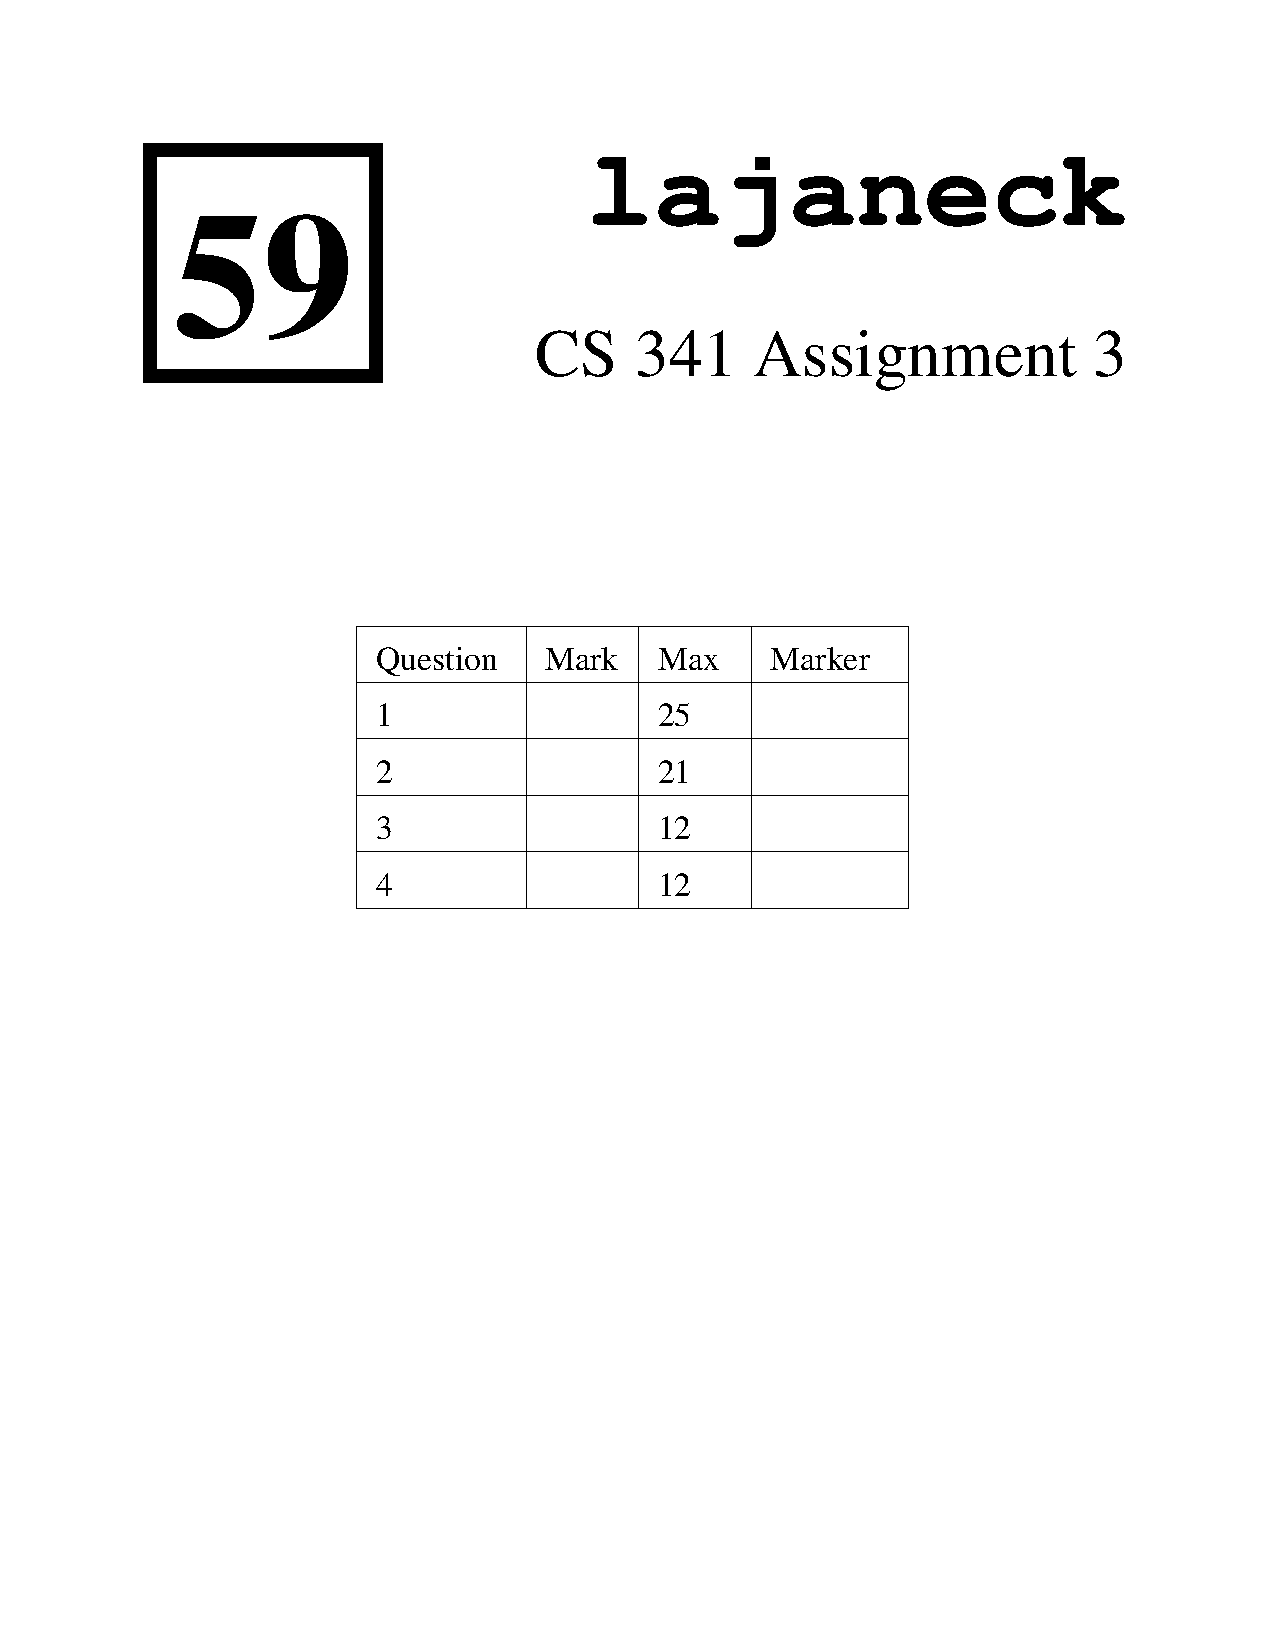
\includepdf[pages={1}]{cover.pdf}


\section*{Question 1a}
\begin{verbatim}
#include <iostream>
#include <fstream>
#include <vector>
#include <math.h>
#include <limits>


struct point {
    int c; //blue == 1
    int x;
    int y;
};

std::pair<int, std::vector<point> > DominanceCount(std::vector<point> A) {
    std::pair<int, std::vector<point> > ret;

    if(A.size() <= 1) {
        ret.first = 0;
        ret.second = A;
        return ret;
    }

    std::vector<point> left;
    left.insert(left.begin(), A.begin(), A.begin() + floor(A.size()/2));
    std::vector<point> right;
    right.insert(right.begin(), A.begin() + ciel(A.size()/2), A.end());

    std::pair<int, std::vector<point> > LeftResult = DominanceCount(left);
    std::pair<int, std::vector<point> > RightResult = DominanceCount(right);

    std::vector<point> L = LeftResult.second;
    std::vector<point> R = RightResult.second;

    point end;
    end.x = std::numeric_limits<int>::max();
    end.y = std::numeric_limits<int>::max();
    end.c = 1;

    L.push_back(end);
    R.push_back(end);

    ret.first += LeftResult.first;
    ret.first += RightResult.first;

    int i = 0;
    int j = 0;
    int blueCount = 0;
    int total = 0;


    for(int k = 0; k < A.size(); k++) {
        point l = L[i];
        point r = R[j];

        if(l.y < r.y) {
            if(l.c == 1) {
                blueCount ++;
            }
            ret.second.push_back(l);
            i++;
        } else {
            if(r.c == 0){
                total += blueCount;
            }
            ret.second.push_back(r);
            j++;
        }
    }


    ret.first += total;
    return ret;
}


int main() {
    int n;
    std::vector<point> A;

    std::cin >> n;
    for(; n > 0; n--){
        point p;

        std::cin >> p.x;
        std::cin >> p.y;
        std::cin >> p.c;

        A.push_back(p);
    }


    std::pair<int, std::vector<point> > result;
    result = DominanceCount(A);
    std::cout << result.first << std::endl;
}

\end{verbatim}

\begin{tabular}{|c|l|l|}
    \hline
    \textbf{n} & \textbf{$\mathcal{O}(n\log{}n)$} & {$\mathcal{O}(n^2)$}\\
    \hline
    10 & 0.00370287895203 & 0.00319194793701 \\
    \hline
    50 & 0.00311994552612 & 0.00292801856995 \\
    \hline
    100 & 0.00425696372986 & 0.00229406356812 \\
    \hline
    150 & 0.00334501266479 & 0.00493001937866 \\
    \hline
    200 & 0.00500988960266 & 0.00331592559814 \\
    \hline
    250 & 0.00591897964478 & 0.00418996810913 \\
    \hline
    300 & 0.00362014770508 & 0.00438213348389 \\
    \hline
    500 & 0.00849390029907 & 0.019513130188 \\
    \hline
    750 & 0.0121681690216 & 0.0274629592896 \\
    \hline
    1000 & 0.00642991065979 & 0.0334718227386 \\
    \hline
\end{tabular}

The input was generated using a random number sampler with range 0-1000 for y values and for x values, and a random integer from 0-1 for color values. The sampler doesn't repeat values so every x and y value is unique. Then sorted the x values and printed each value in sets of three to an output file. The above inputs show that for smaller inputs the $\mathcal{O}(n^2)$ algorithm is faster. This is primarily due to the overhead accrued from the more complex data structures and calculations used in the $\mathcal{O}(n\log{}n)$ algorithm. For all inputs greater than roughly 250 the $\mathcal{O}(n\log{}n)$ algorithm is faster as can be expected.

\section*{Question 2}
\subsection*{a)}
\begin{center}
\begin{algorithm}
    mailbox = $houses_0$ + D\;
    i = 0\;
    \textbf{sort} houses\;
    \While{i $\leq$ n}{
        \If{$x_i$ $>$ mailbox + D}{
            build a mailbox at mailbox\;
            mailbox = $houses_i$ + D\;
            i ++\;
        }
    }
\end{algorithm}
\end{center}
Here we iterate through the array houses and any time a house is not within D of the most recently placed mailbox (denoted ``mailbox'') a new mailbox is placed with this house at the left most edge of its range. And since we iterate through the house array touching each house once its time complexity is is $\sum_{i=1}^n = \mathcal{O}(nc) = \mathcal{O}(n)$, but since the algorithm starts by sorting the houses its time complexity is $\mathcal{O}(n\log n)$.

\subsection*{b)}
\textbf{solution is feasibility}:\\
    Since the algorithm checks for houses outside of the mailboxes range and adds a mailbox to cover it, there cannot be house outside of a mailbox's range.

\textbf{solution is optimal}:\\
    Let m* be the number of mailboxes in a an optimal solution, Let m be the number of mailboxes in our solution.\\
    Suppose m* $<$ m. This means that there are mailboxes in m that could have been removed. Say mailbox mail could be removed to make m == m* while maintaining feasibility. This means that mail has no houses in its range that are not covered by another mail box. In line 5 of the algorithm it checks for houses more than D away from a mailbox then places a mailbox D from them. This means that mailboxes are more then 2D away from each other so a mailbox cannot overlap another mailbox's range. Similarly each mailbox is placed at $houses_i$ + D so each mailbox must be in range of at least one house. This means that mail must have at least one house in its range, and its range cannot overlap with another mailbox. If mail was removed the house in its range wouldn't be covered. So there is no mailbox in m that can be removed to make m* so m == m* or m* would not be feasible.

\subsection*{c)}
\begin{tabular}{|l|l|l|l|}
    \hline
    \textbf{i} & \textbf{mailboxes} & \textbf{covered houses} & \textbf{uncovered houses}\\
    \hline
    0 & -7, & -10 & -8, -5, -2, -1, 1, 2, 4, 5, 8, 11, 12, 14, 16, 19\\
    \hline
    1 & -7 & -10, -8 & -5, -2, -1, 1, 2, 4, 5, 8, 11, 12, 14, 16, 19\\
    \hline
    1 & -7 & -10, -8, -5 & -2, -1, 1, 2, 4, 5, 8, 11, 12, 14, 16, 19\\
    \hline
    2 & -7, 1 & -10, -8, -5, -2 & -1, 1, 2, 4, 5, 8, 11, 12, 14, 16, 19\\
    \hline
    3 & -7, 1 & -10, -8, -5, -2, -1 & 1, 2, 4, 5, 8, 11, 12, 14, 16, 19\\
    \hline
    4 & -7, 1 & -10, -8, -5, -2, -1, 1, 2 & 4, 5, 8, 11, 12, 14, 16, 19\\
    \hline
    5 & -7, 1 & -10, -8, -5, -2, -1, 1, 2, 4 & 5, 8, 11, 12, 14, 16, 19\\
    \hline
    6 & -7, 1, 8 & -10, -8, -5, -2, -1, 1, 2, 4, 5 & 8, 11, 12, 14, 16, 19\\
    \hline
    7 & -7, 1, 8 & -10, -8, -5, -2, -1, 1, 2, 4, 5, 8 & 11, 12, 14, 16, 19\\
    \hline
    8 & -7, 1, 8 & -10, -8, -5, -2, -1, 1, 2, 4, 5, 8, 11 & 12, 14, 16, 19\\
    \hline
    9 & -7, 1, 8, 15 & -10, -8, -5, -2, -1, 1, 2, 4, 5, 8, 11, 12 & 14, 16, 19\\
    \hline
    10 & -7, 1, 8, 15 & -10, -8, -5, -2, -1, 1, 2, 4, 5, 8, 11, 12, 14 & 16, 19\\
    \hline
    11 & -7, 1, 8, 15 & -10, -8, -5, -2, -1, 1, 2, 4, 5, 8, 11, 12, 14, 16 & 19\\
    \hline
    12 & -7, 1, 8, 15, 22 & -10, -8, -5, -2, -1, 1, 2, 4, 5, 8, 11, 12, 14, 16, 19 & \\
    \hline
\end{tabular}


\section*{Question 3}
\subsection*{a)}
Let $T_{prev}$ be the running total in the previous iteration of the for loop. At that point in time we also know that $x_{j-1} = \bigg \lfloor \frac{T_{prev}}{d_{j-1}} \bigg \rfloor$ as that was the equation used for calculating the previous x value.
\begin{align*}
    T &= T_{prev} - x_{j-1} d_{j-1}\\
        &= T_{prev} - \bigg \lfloor \frac{T_{prev}}{d_{j-1}} \bigg \rfloor d_{j-1}\\
        &\leq T_{prev} - \bigg ( \frac{T_{prev}}{d_{j-1}} - 1 \bigg ) d_{j-1}\\
        &\leq T_{prev} - T_{prev} + d_{j-1}\\
        &\leq d_{j-1}\\
    x_j &= \bigg \lfloor \frac{T}{d_j} \bigg \rfloor\\
    x_j &\leq \bigg \lfloor \frac{d_{j-1}}{d_j} \bigg \rfloor\\
    x_j &\leq \frac{d_{j-1}}{d_j} - 1
\end{align*}


\subsection*{b)}
\begin{align*}
    0 \leq x_j^* & \leq \frac{d_{j-1}}{d_j} -1
\end{align*}
Since $d_{j-1}$ is divisible by $d_j$ Let $d_{j-1} = ad_j$
\begin{align*}
    0 \leq x_j^* & \leq \frac{ad_{j}}{d_j}-1 \\
    0 \leq x_j^* & \leq a - 1 \\
\end{align*}
Since $x_j^*$ is an integer
\begin{align*}
    0 \leq x_j^* & < a
\end{align*}
This is true, when $x_j^* \geq a$ we can exchange $ad_j$ for $1d_{j-1}$to lower our N which isnt possible in an optimal solution.

\subsection*{c)}
Since both solutions must be feasible they must also both sum to T.
\begin{align*}
    T=\sum_{j=1}^n x_j d_j &= \sum_{j=1}^n x_j^* d_j
\end{align*}
Since i is the highest index where $x^*_i \not = x_i$ we know that all values after it must be equal.
\begin{align*}
    \text{Let }\delta = \sum_{j=i+1}^n x_j d_j &= \sum_{j=i+1}^n x_j^* d_j
\end{align*}
So our analysis deals only with the elements before i
\begin{align*}
    T - \delta=\sum_{j=1}^i x_j d_j &= \sum_{j=1}^i x_j^* d_j\\
                \sum_{j=1}^{i-1} x_j d_j  + x_i d_i&= \sum_{j=1}^{i-1} x_j^* d_j + x_i^* d_i\\
                \sum_{j=1}^{i-1} x_j d_j  + d_i(x_i - x_i^*)&= \sum_{j=1}^{i-1} x_j^* d_j
\end{align*}
We can continue to repeat this process of separating out the highest term and subtracting from both sides
\begin{align*}
    \sum_{j=1}^{i-1} x_j d_j  + d_i(x_i - x_i^*) &= \sum_{j=1}^i x_j^* d_j\\
    \sum_{j=1}^{i-2} x_j d_j  + d_i(x_i - x_i^*)  + x_{i-1} d_{i-1}&= \sum_{j=1}^{i-2} x_j^* d_j + x_{i-1}^* d_{i-1}\\
    \sum_{j=1}^{i-1} x_j d_j  + d_i(x_i - x_i^*) + d_{i-1}(x_{i-1} - x_{i-1}^*)&= \sum_{j=1}^{i-2} x_j^* d_j\\
    \dots\\
    \sum_{j=1}^{i} d_j(x_j - x_j^*) &= 0
\end{align*}
Using the previous parts we can find a bound for $x_j - x_j^*$. We know that it must be greater than 0 since $x_j \not = x_j^*$ and the greedy algorithm always takes the greatest $x_j$. We can also say that the largest possible value is when $x_j$ is at its max of $\frac{d_{j-1}}{d_j} - 1$ and $x_j^*$ is at its min of 0. So let $x_j - x_j^* = \epsilon$ where $\epsilon$ is a trivially small non-zero number.
\begin{align*}
    \sum_{j=1}^{i} d_j(x_j - x_j^*) &= \sum_{j=1}^{i} d_j \epsilon\\
                                    &> 0
\end{align*}
This is a contradiction. The only possible way to make this work is for $x_j = x_j^*$ for all values of j.

This means that the greedy algorithm will always return an optimal solution.


\section*{Question 4}
\subsection*{a)}
For each element j in I, find the median element of I, at i. If $s_j$ (starting value of j) is greater than or equal to $f_i$ (ending value of i) recurse on the left half of I, else recurse on the right half of I. Once there is one element return the index of that element. This takes $O(\log n)$ like a binary search, so when you repeat it for each element it is $O(n\log n)$

\subsection*{b)}
If I[j] is in the optimal solution then its profit should the be profit of the closest not overlapping interval given by the last function, and its own profit which is $p_j + P(\text{last(j)})$. A special case must be made if last(j) = 0 which should just return the profit of I[j]. If I[j] is not in the optimal solution then the value is just the profit of the previous one, $P(j-1)$. To maximize the solution we take the max of these two values resulting in $\max \{ p_j + P(\text{last(j)}), P(j-1)\}$.

So the maximal recurrence is:
\begin{align*}
    P(0) &= 0\\
    f(j) &= \begin{cases}
    p_j & \text{if last}(j) = 0\\
    p_j + P(\text{last}(j)) & \text{else}
    \end{cases}\\
    &\max \{f(j), P(j-1)\}
\end{align*}

\subsection*{c)}
\begin{center}
\begin{tabular}{c c c c c c}
    interval & [$s_j,f_j$) & $p_j$ & last(j) & P(j)\\
    \hline
    $I_1$ & [2,3) & 2 & 0 & 2\\
    $I_2$ & [2,4) & 3 & 0 & $\max \{ 3, 2\}$ = 3\\
    $I_3$ & [1,6) & 5 & 0 & $\max \{ 5, 3\}$ = 5\\
    $I_4$ & [3,8) & 4 & 1 & $\max \{ 4 + P(1), P(3)\}$ = $\max \{ 6, 5\}$ = 6\\
    $I_5$ & [4,9) & 4 & 2 & $\max \{ 4 + P(2), P(4)\}$ = $\max \{ 7, 6\}$ = 7\\
    $I_6$ & [6,11) & 1 & 3 & $\max \{ 1 + P(3), P(5)\}$ = $\max \{ 6, 7\}$ = 7\\
    $I_7$ & [5,12) & 3 & 2 & $\max \{ 3 + P(2), P(6)\}$ = $\max \{ 6, 7\}$ = 7\\
    $I_8$ & [12,13) & 1 & 7 & $\max \{ 1 + P(7), P(7)\}$ = $\max \{ 8, 7\}$ = 8\\
    $I_9$ & [9,14) & 3 & 5 & $\max \{ 3 + P(<5), P(8)\}$ = $\max \{ 10, 8\}$ = 10\\
    $I_{10}$ & [11,15) & 2 & 6 & $\max \{ 2 + P(6), P(9)\}$ = $\max \{ 9, 10\}$ = 10\\
    $I_{11}$ & [14,16) & 2 & 9 &  $\max \{ 2 + P(9), P(10)\}$ = $\max \{ 12, 10\}$ = 12\\
    $I_{12}$ & [13,18) & 4 & 8 & $\max \{ 4 + P(8), P(11)\}$ = $\max \{11 , 12\}$ = 12\\
\end{tabular}
\end{center}
$P(n) = \bigg\{\{2, 5, 8, 12\}, \{2, 5, 9, 11\}\bigg\}$

\end{document}
